\section{Results for Part II}

In this section I will show:
\begin{itemize}
  \item how I decided to conduct tests for the part of the assignment related
    to meta-heuristic;
  \item some statistics, i.e. minimum, maximum, mean of the objective function.
\end{itemize}

\subsection{Scenarios}

As I did for the tests of the Part I, I prepared a bit of configuration also
to test the program that uses the genetic algorithm.

In fact, I automatized the tests to run by combining the settings shown in
\ref{sec:resI-scenarios} with the tuning I made for the algorithm (see
\ref{sec:par-calib}).

So, I tested all the scenarios (\textit{345}, \textit{tsp12}, \textit{tsp60},
\textit{gerber}, \textit{ru}, \textit{rg} and \textit{rg\_Manh}) with all the
configurations shown in Table \ref{tab:settings}, running the algorithm at
least seven times with each of the following calibrations\footnote{all the
tests were run with a population size of $55$}:

\begin{table}[H]
  \centering
  \begin{tabular}{|l|c|c|c|r|}
    \hline
    \textbf{\textit{name}} & \textbf{\textit{t}} (s) & \textbf{\textit{m}} &
    \textbf{\textit{h}} & \textbf{\textit{e}} \\
    \hline
    \hline
    Avg & $5.0$ & $50\%$ & 5 & 3 \\
    \hline
    BE & $5.0$ & $50\%$ & 5 & 20 \\
    \hline
    Mut & $5.0$ & $100\%$ & 5 & 3 \\
    \hline
    NH & $5.0$ & $50\%$ & 0 & 3 \\
    \hline
    Time & $60.0$ & $50\%$ & 5 & 3 \\
    \hline
  \end{tabular}
  \caption{Parameter tuning for Part II tests}
  \label{tab:tuning}
\end{table}

Where:
\begin{itemize}
  \item $t$ stands for \textit{time limit};
  \item $m$ stands for \textit{mutation probability};
  \item $h$ stands for \textit{initial population generated with Simulated
    Annealing};
  \item $e$ stands for \textit{elite size}.
\end{itemize}

\subsection{Part II performance}

Hereafter, I show some box plots that depict how the objective function value
was computed by the genetic algorithm with different configurations.

\paragraph{Note} Data for the \textit{345} instance is omitted since it was so
simple to solve that all the runs always yielded the optimum value.

\paragraph{Note} Data and charts for variances are not displayed since you can
already figure out (arguably) well how much the performance varied from the box
plots.

%%%%%%%%%%%%%%%%%%%
%% FIXED
%%%%%%%%%%%%%%%%%%%

\begin{figure}[H]

\begin{minipage}{.5\linewidth}
\centering
\subfloat[]{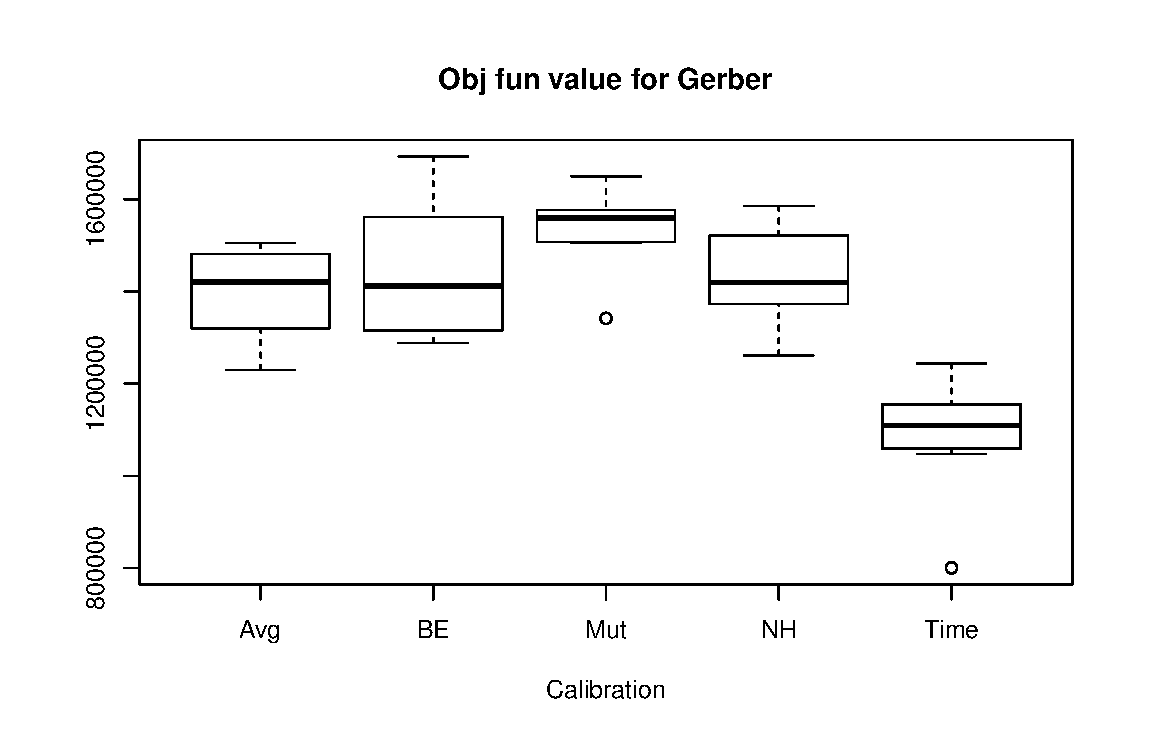
\includegraphics[scale=.4]{pics/boxplots/gerber.eps}}
\end{minipage}%
\begin{minipage}{.5\linewidth}
\centering
\subfloat[]{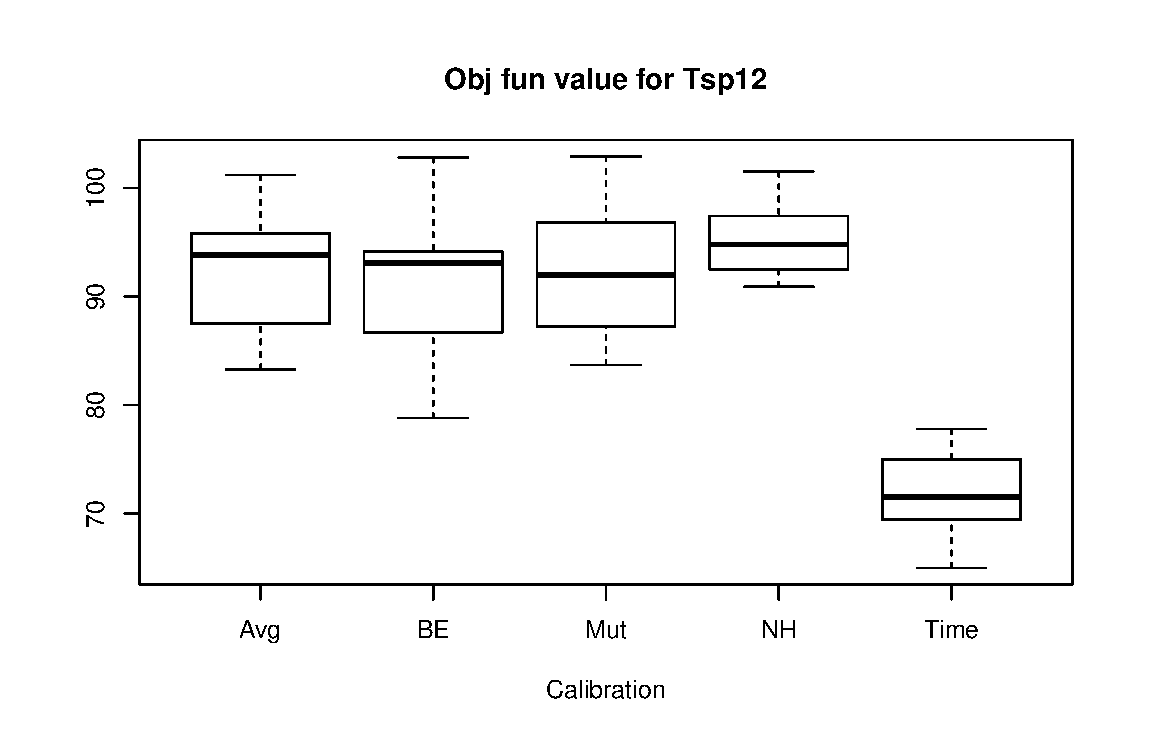
\includegraphics[scale=.4]{pics/boxplots/tsp12.eps}}
\end{minipage}\par\medskip
\centering
\subfloat[]{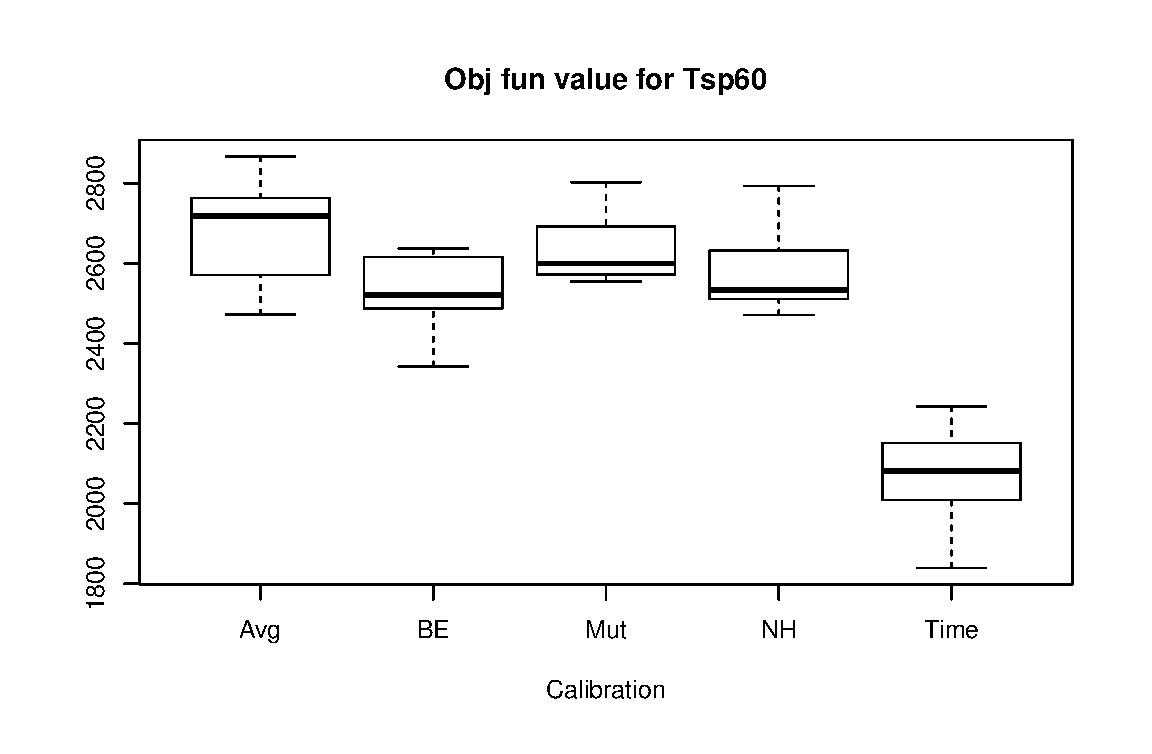
\includegraphics[scale=.4]{pics/boxplots/tsp60.eps}}

\caption{Objective function performance on fixed instances}
\label{fig:obj-fixed}
\end{figure}

%%%%%%%%%%%%%%%%%%%
%% RU 10 holes
%%%%%%%%%%%%%%%%%%%

\begin{figure}[H]

\begin{minipage}{.5\linewidth}
\centering
\subfloat[]{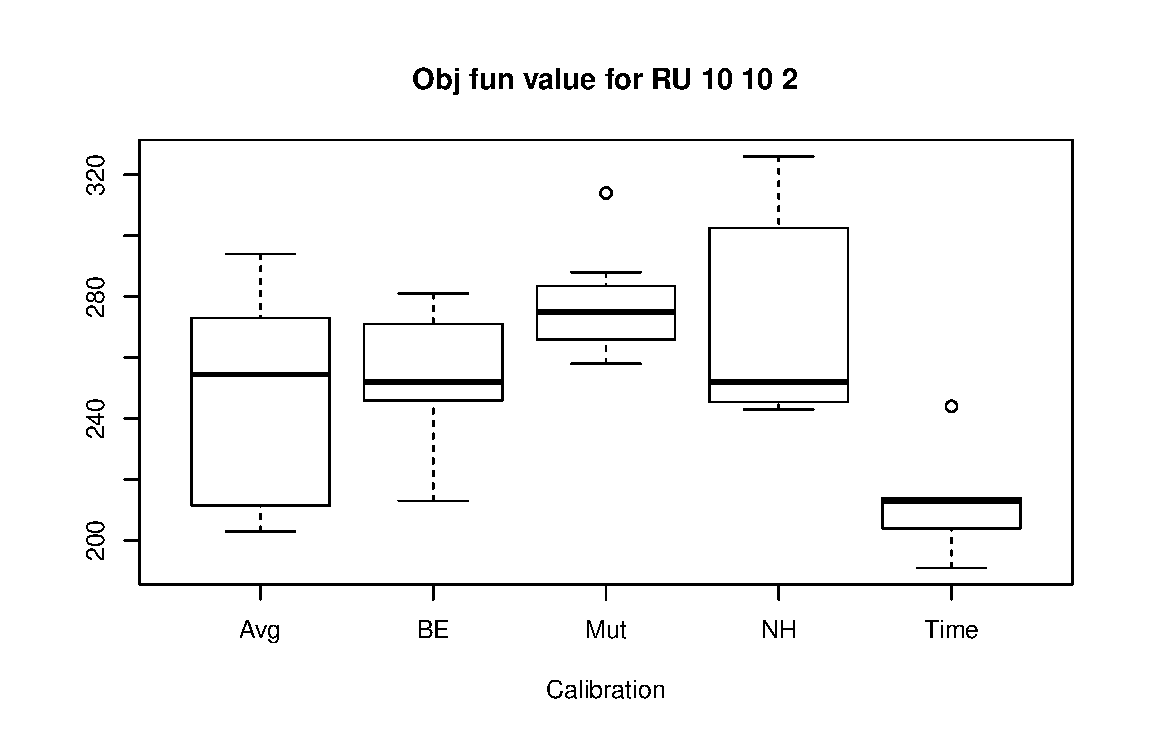
\includegraphics[scale=.4]{pics/boxplots/ru-10-10-2.eps}}
\end{minipage}%
\begin{minipage}{.5\linewidth}
\centering
\subfloat[]{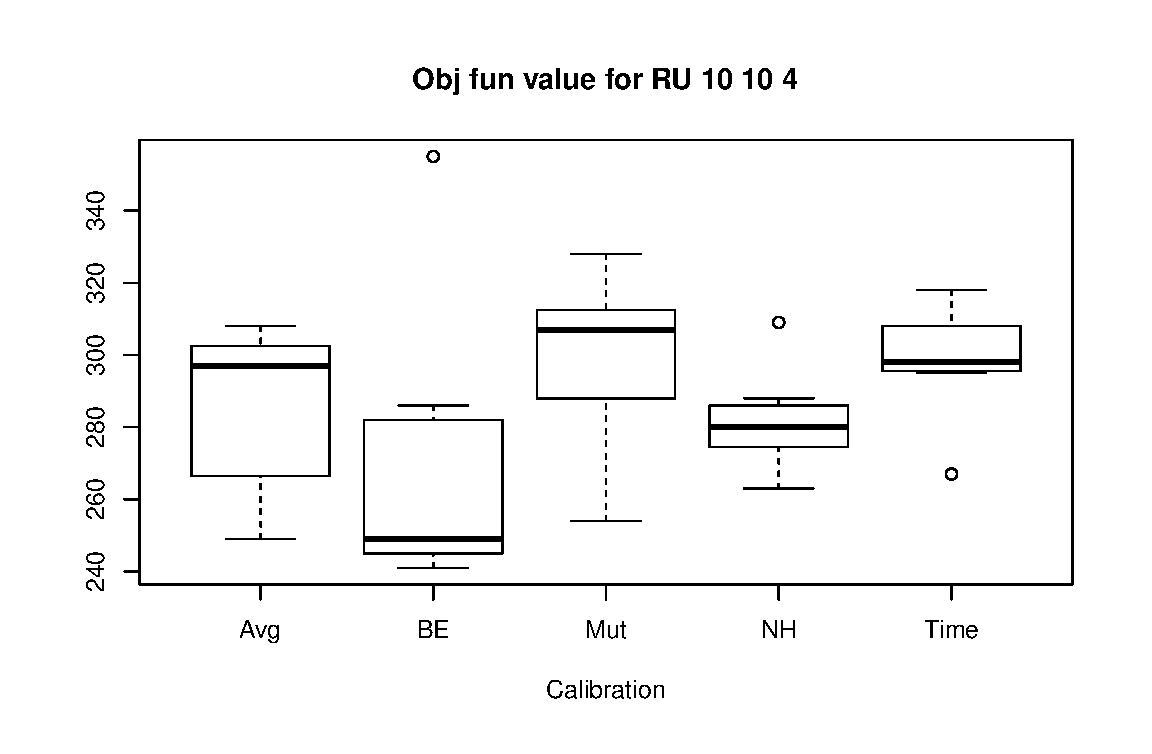
\includegraphics[scale=.4]{pics/boxplots/ru-10-10-4.eps}}
\end{minipage}\par\medskip
\centering
\begin{minipage}{.5\linewidth}
\centering
\subfloat[]{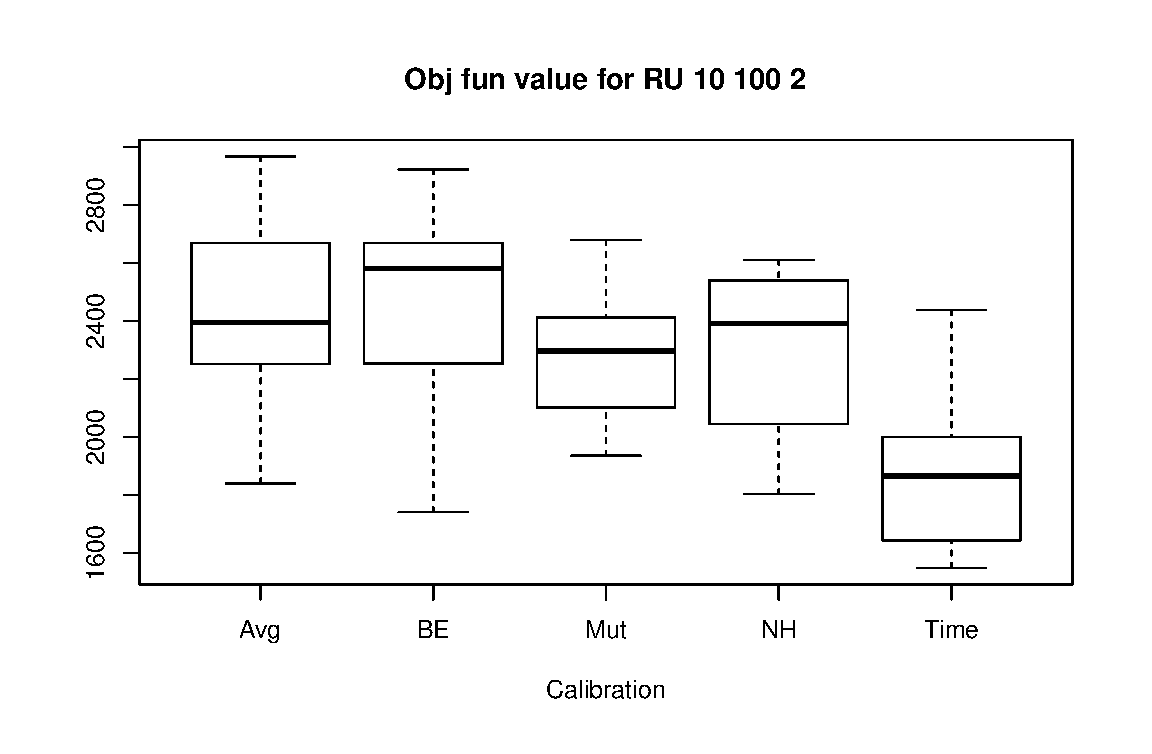
\includegraphics[scale=.4]{pics/boxplots/ru-10-100-2.eps}}
\end{minipage}%
\begin{minipage}{.5\linewidth}
\centering
\subfloat[]{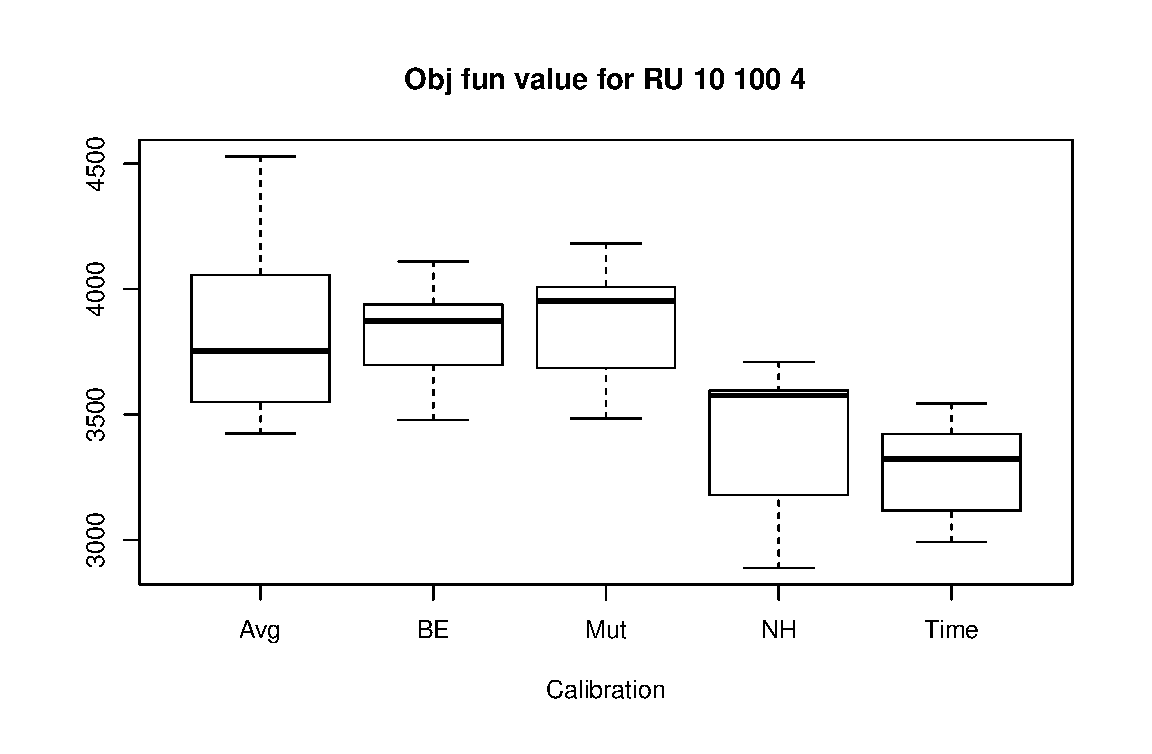
\includegraphics[scale=.4]{pics/boxplots/ru-10-100-4.eps}}
\end{minipage}\par\medskip

\caption{Objective function performance for Random Uniform with 10 holes}
\label{fig:obj-fixed}
\end{figure}

%%%%%%%%%%%%%%%%%%%
%% RU 50 holes
%%%%%%%%%%%%%%%%%%%

\begin{figure}[H]

\begin{minipage}{.5\linewidth}
\centering
\subfloat[]{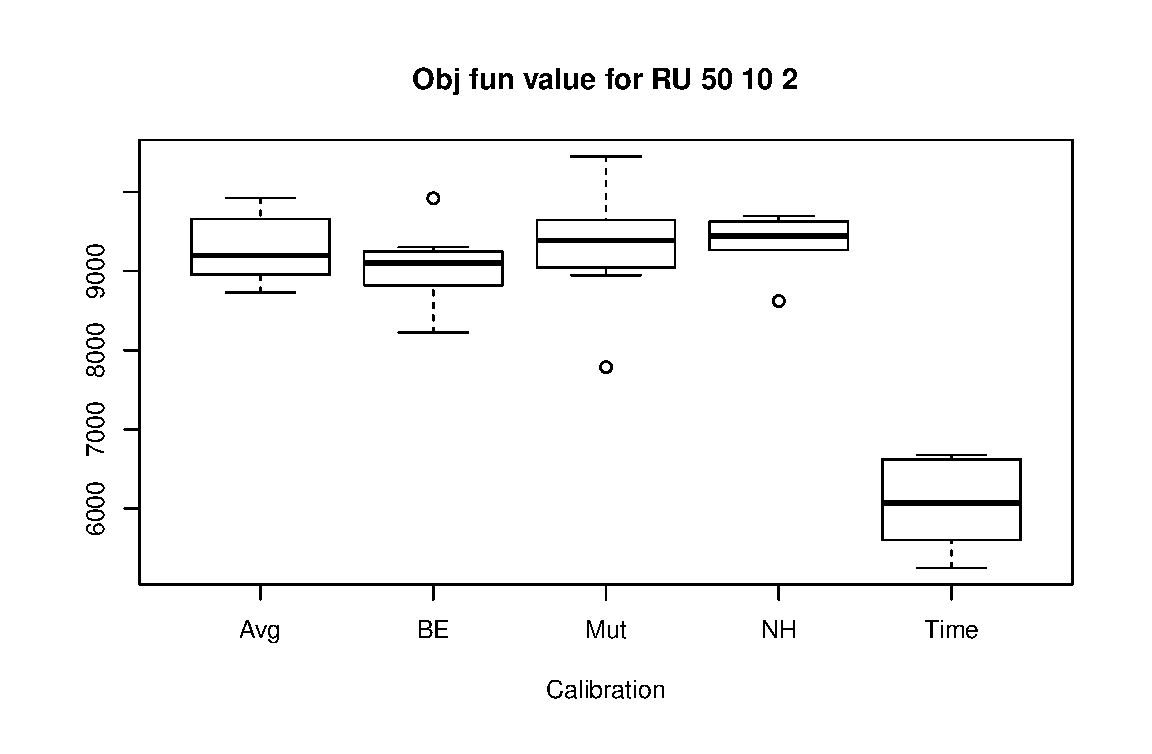
\includegraphics[scale=.4]{pics/boxplots/ru-50-10-2.eps}}
\end{minipage}%
\begin{minipage}{.5\linewidth}
\centering
\subfloat[]{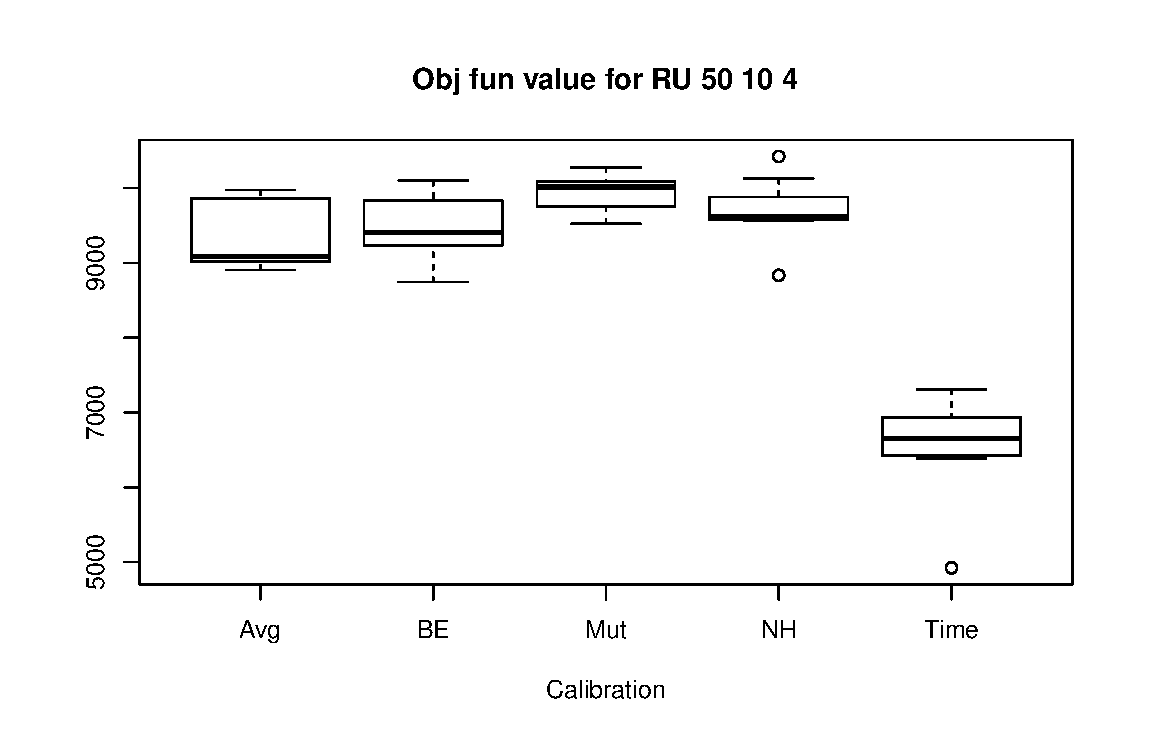
\includegraphics[scale=.4]{pics/boxplots/ru-50-10-4.eps}}
\end{minipage}\par\medskip
\centering
\begin{minipage}{.5\linewidth}
\centering
\subfloat[]{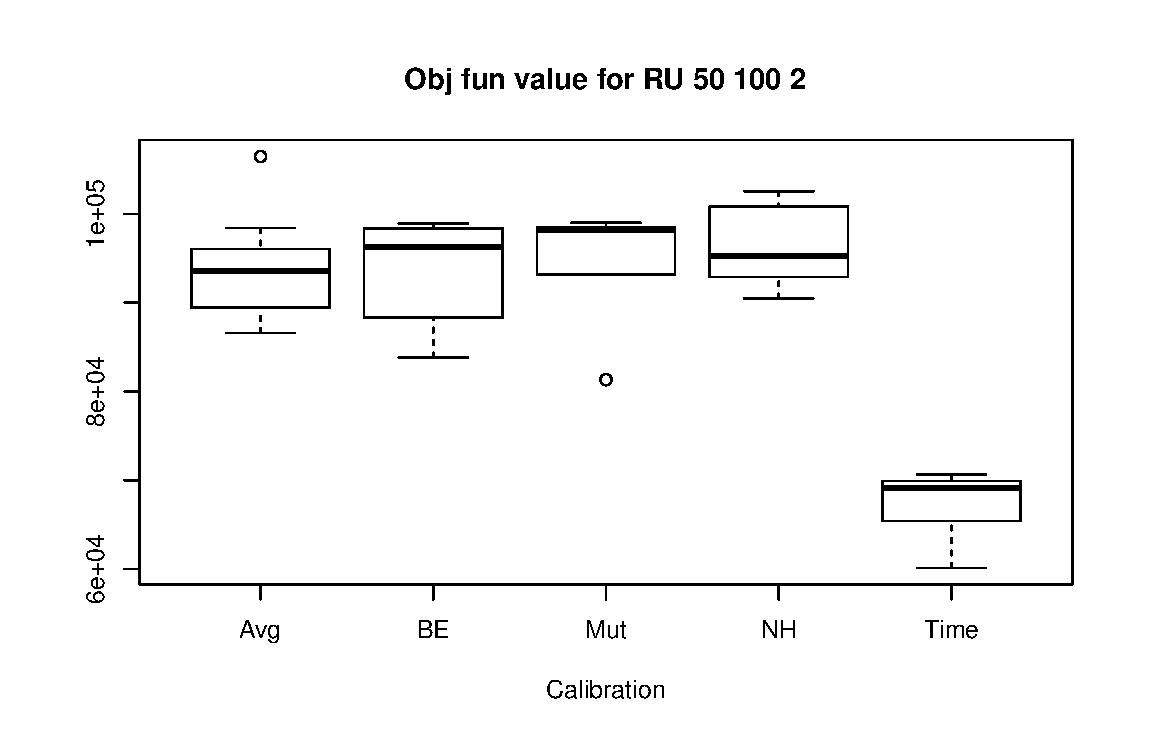
\includegraphics[scale=.4]{pics/boxplots/ru-50-100-2.eps}}
\end{minipage}%
\begin{minipage}{.5\linewidth}
\centering
\subfloat[]{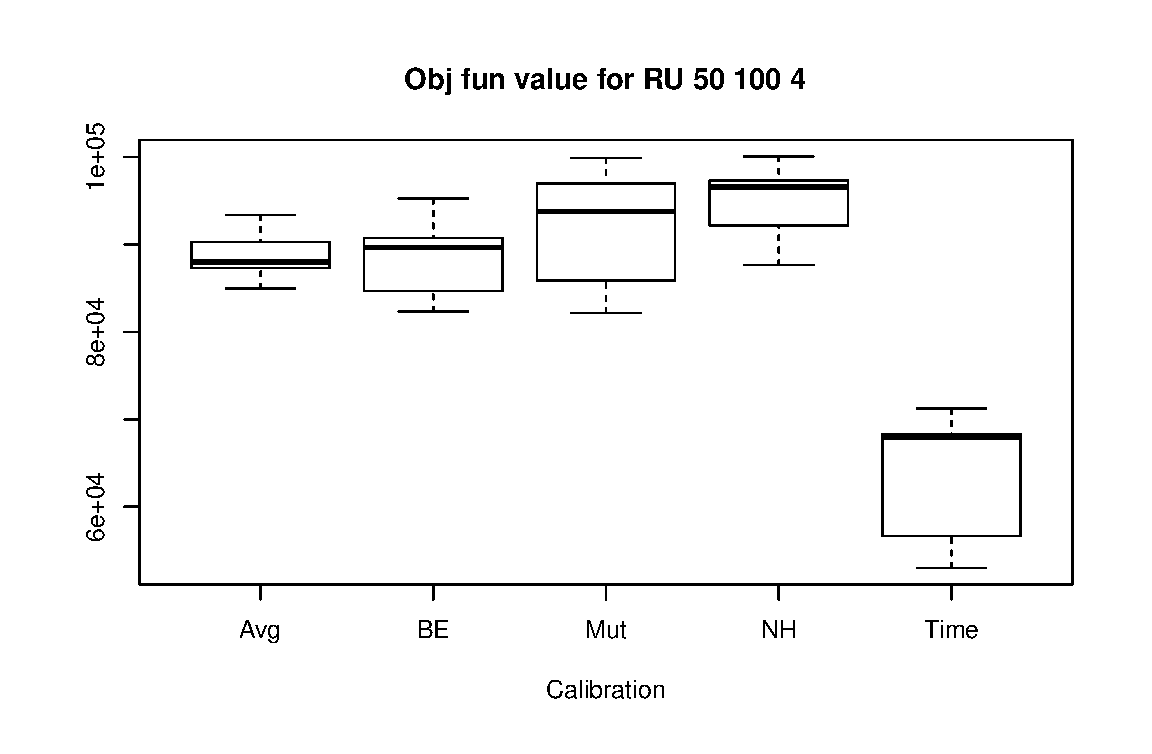
\includegraphics[scale=.4]{pics/boxplots/ru-50-100-4.eps}}
\end{minipage}\par\medskip

\caption{Objective function performance for Random Uniform with 50 holes}
\label{fig:obj-fixed}
\end{figure}

%%%%%%%%%%%%%%%%%%%
%% RG 10 holes
%%%%%%%%%%%%%%%%%%%

\begin{figure}[H]

\begin{minipage}{.5\linewidth}
\centering
\subfloat[]{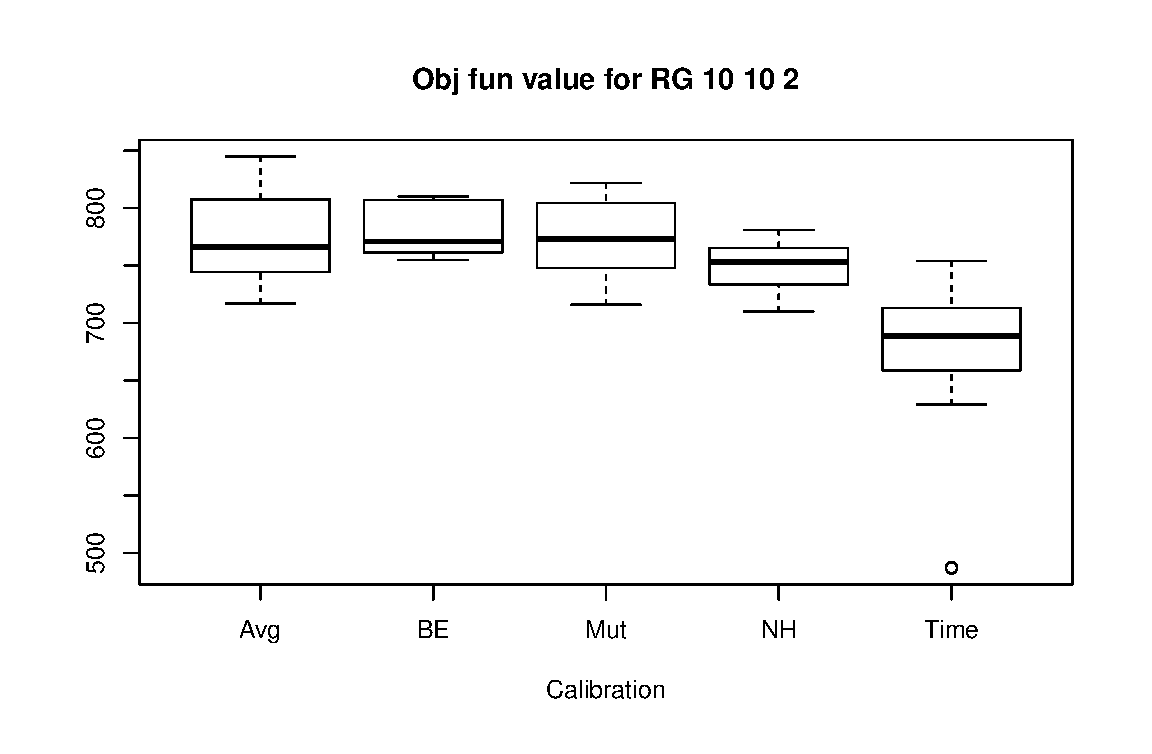
\includegraphics[scale=.4]{pics/boxplots/rg-10-10-2.eps}}
\end{minipage}%
\begin{minipage}{.5\linewidth}
\centering
\subfloat[]{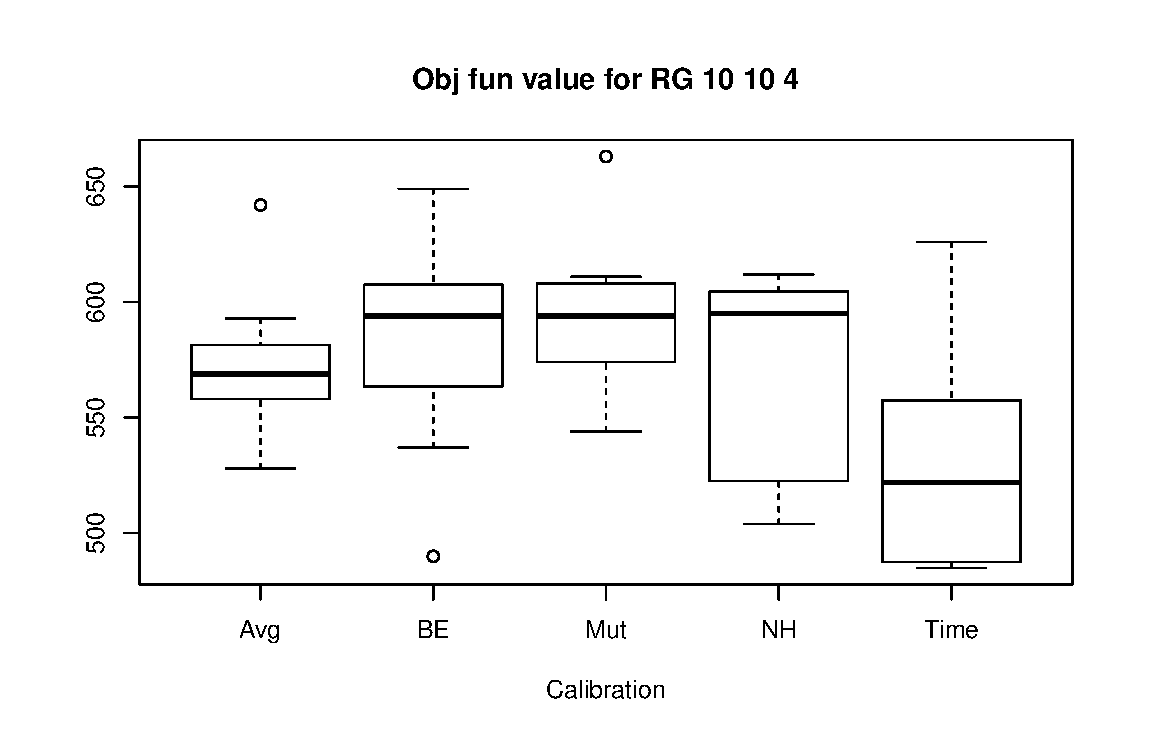
\includegraphics[scale=.4]{pics/boxplots/rg-10-10-4.eps}}
\end{minipage}\par\medskip
\centering
\begin{minipage}{.5\linewidth}
\centering
\subfloat[]{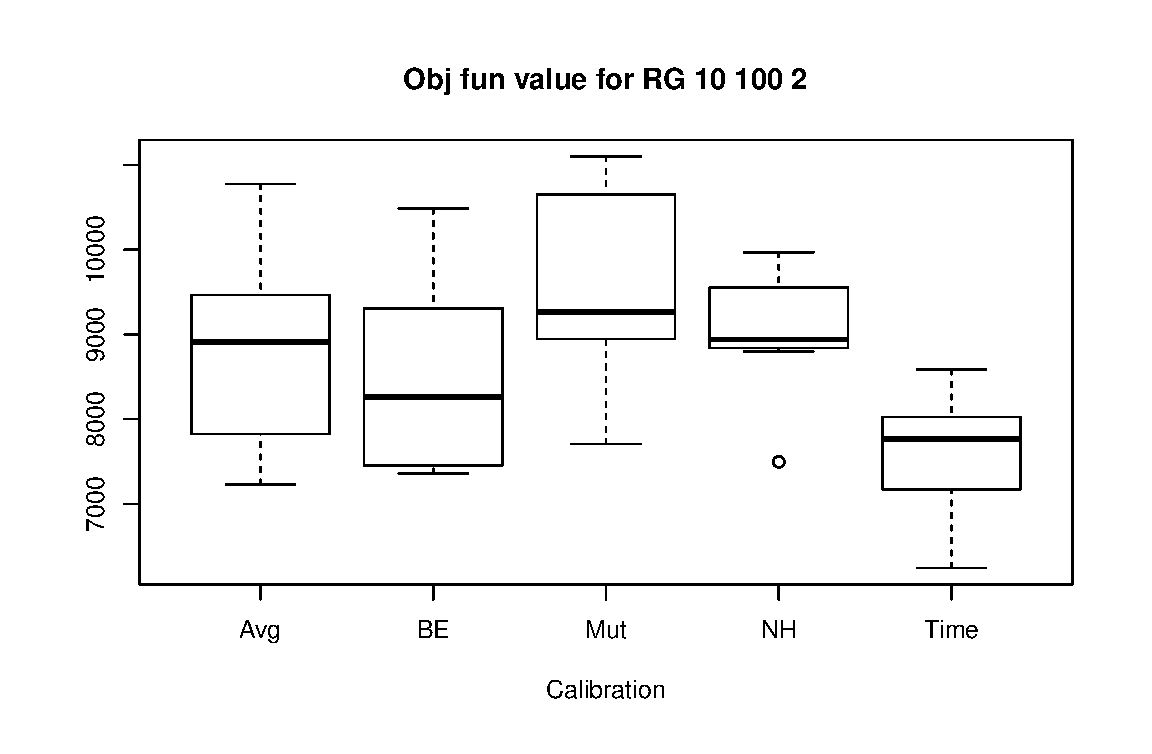
\includegraphics[scale=.4]{pics/boxplots/rg-10-100-2.eps}}
\end{minipage}%
\begin{minipage}{.5\linewidth}
\centering
\subfloat[]{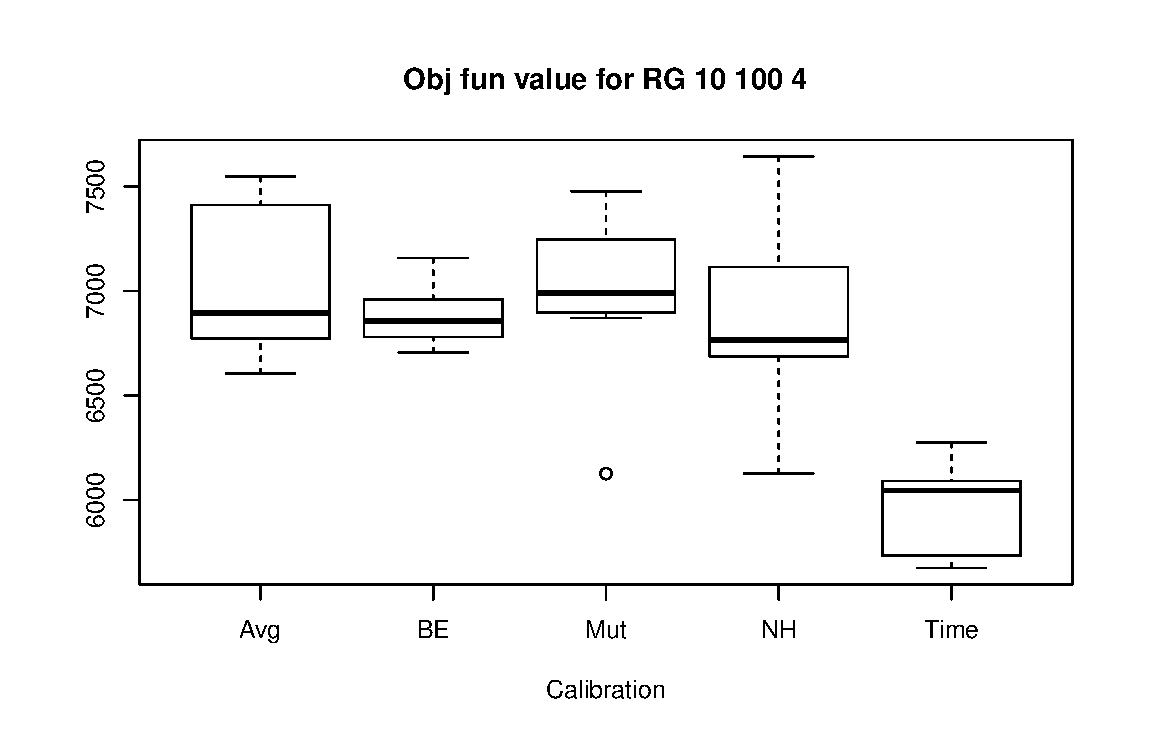
\includegraphics[scale=.4]{pics/boxplots/rg-10-100-4.eps}}
\end{minipage}\par\medskip

\caption{Objective function performance for Random Grid Uniform with 10 holes}
\label{fig:obj-fixed}
\end{figure}


%%%%%%%%%%%%%%%%%%%
%% RG 50 holes
%%%%%%%%%%%%%%%%%%%

\begin{figure}[H]

\begin{minipage}{.5\linewidth}
\centering
\subfloat[]{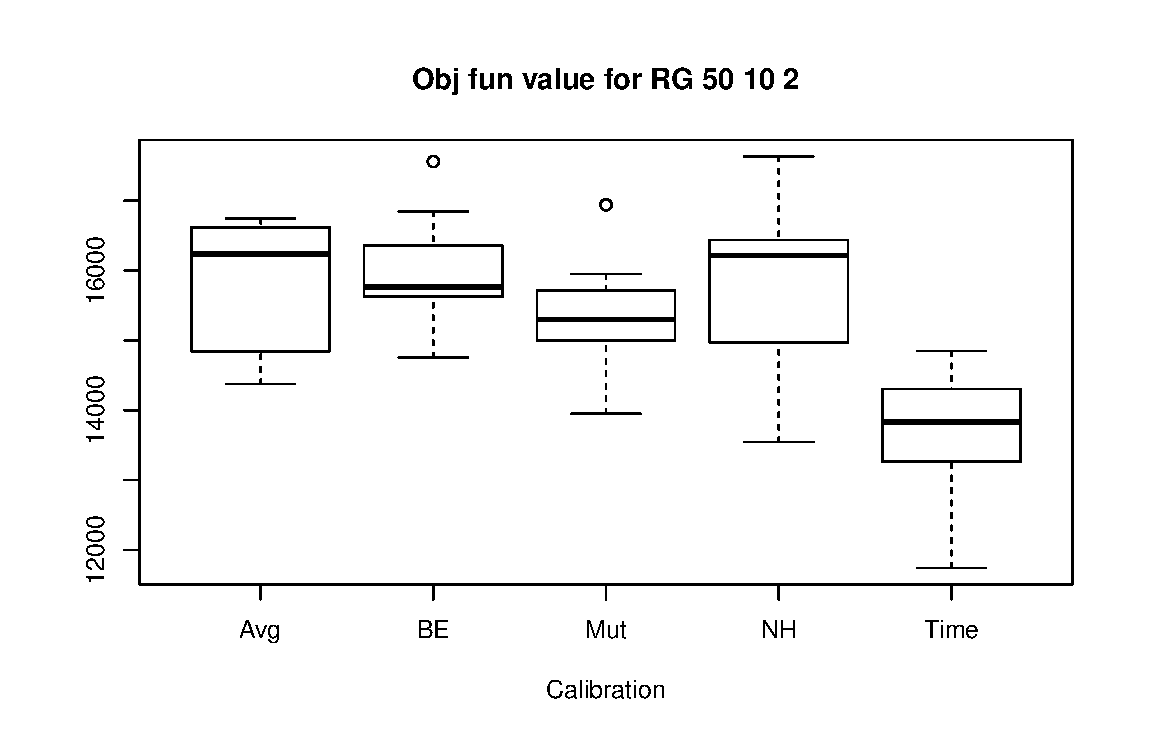
\includegraphics[scale=.4]{pics/boxplots/rg-50-10-2.eps}}
\end{minipage}%
\begin{minipage}{.5\linewidth}
\centering
\subfloat[]{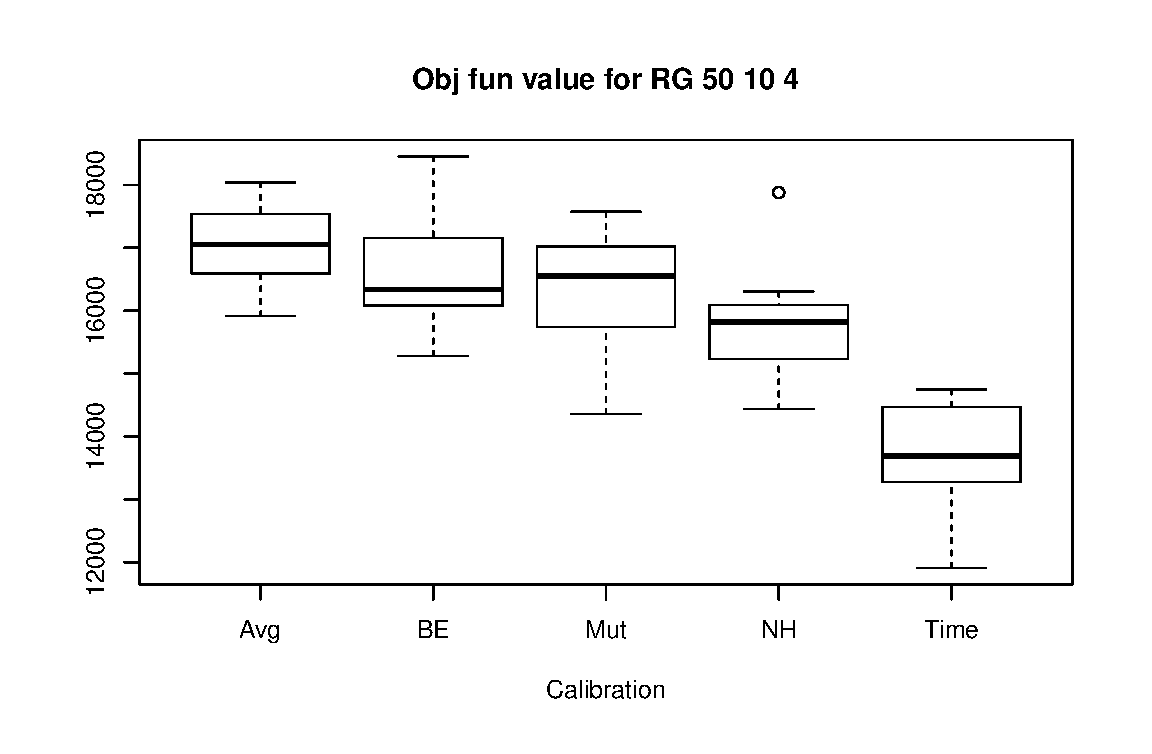
\includegraphics[scale=.4]{pics/boxplots/rg-50-10-4.eps}}
\end{minipage}\par\medskip
\centering
\begin{minipage}{.5\linewidth}
\centering
\subfloat[]{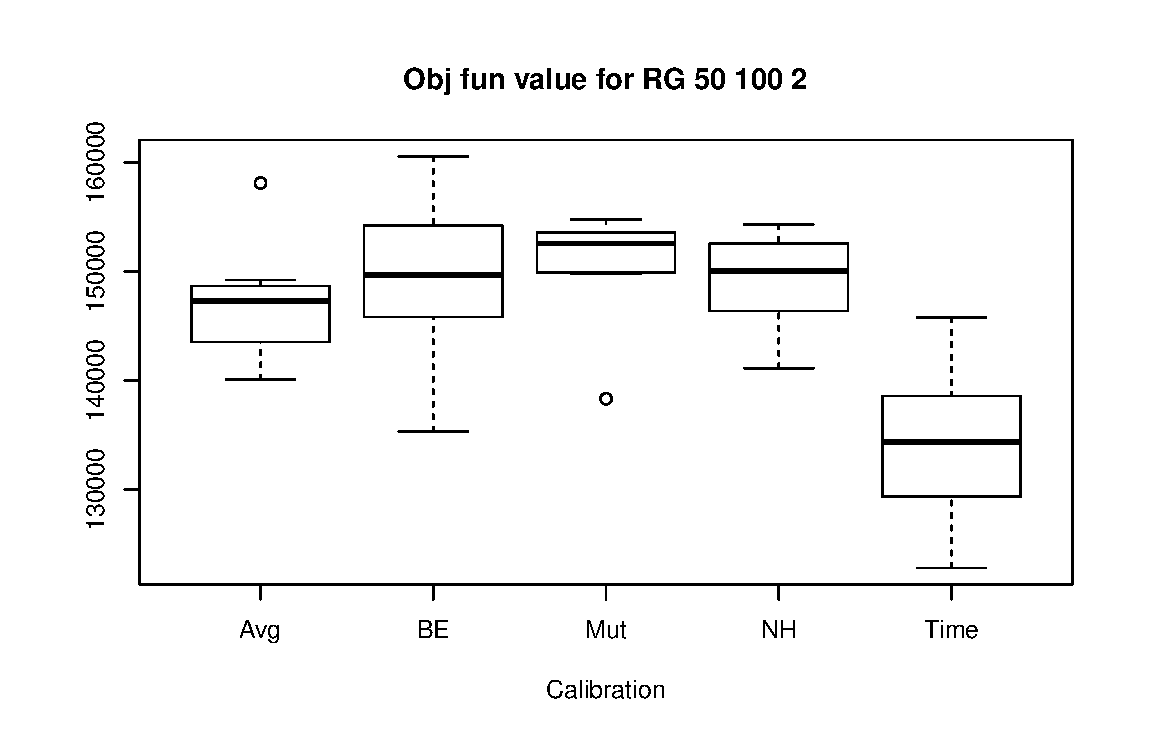
\includegraphics[scale=.4]{pics/boxplots/rg-50-100-2.eps}}
\end{minipage}%
\begin{minipage}{.5\linewidth}
\centering
\subfloat[]{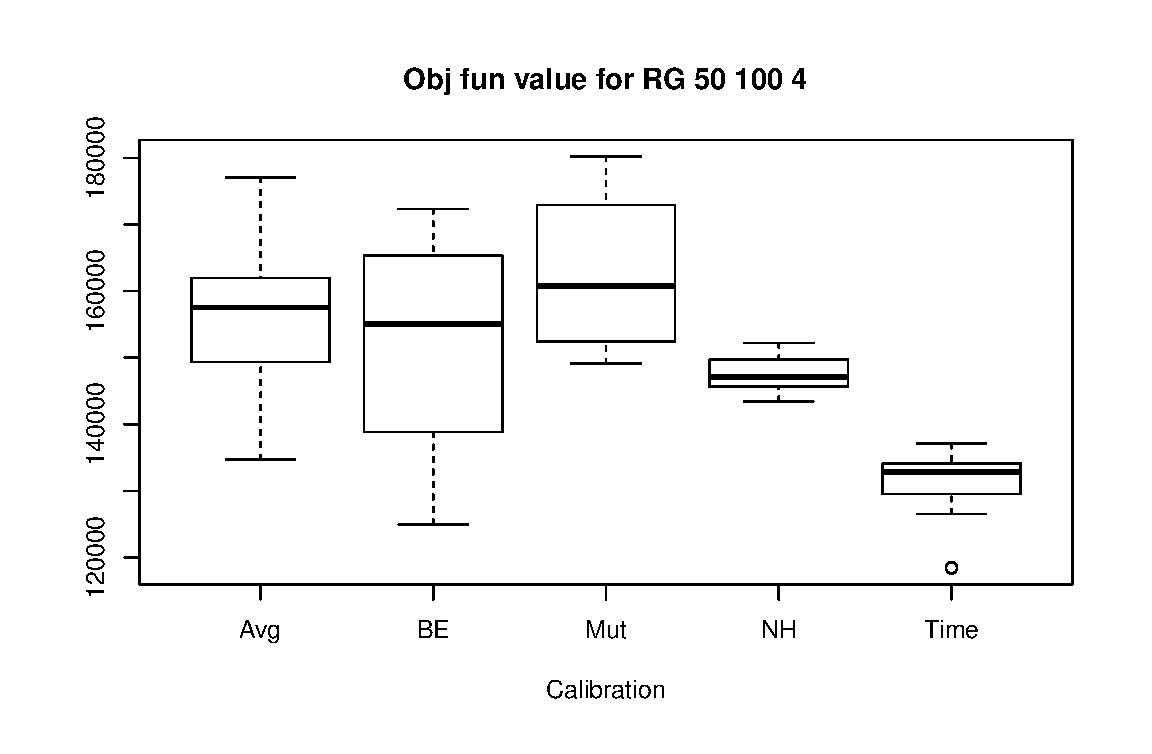
\includegraphics[scale=.4]{pics/boxplots/rg-50-100-4.eps}}
\end{minipage}\par\medskip

\caption{Objective function performance for Random Grid Uniform with 50 holes}
\label{fig:obj-fixed}
\end{figure}


%%%%%%%%%%%%%%%%%%%
%% RG MANH 10 holes
%%%%%%%%%%%%%%%%%%%

\begin{figure}[H]

\begin{minipage}{.5\linewidth}
\centering
\subfloat[]{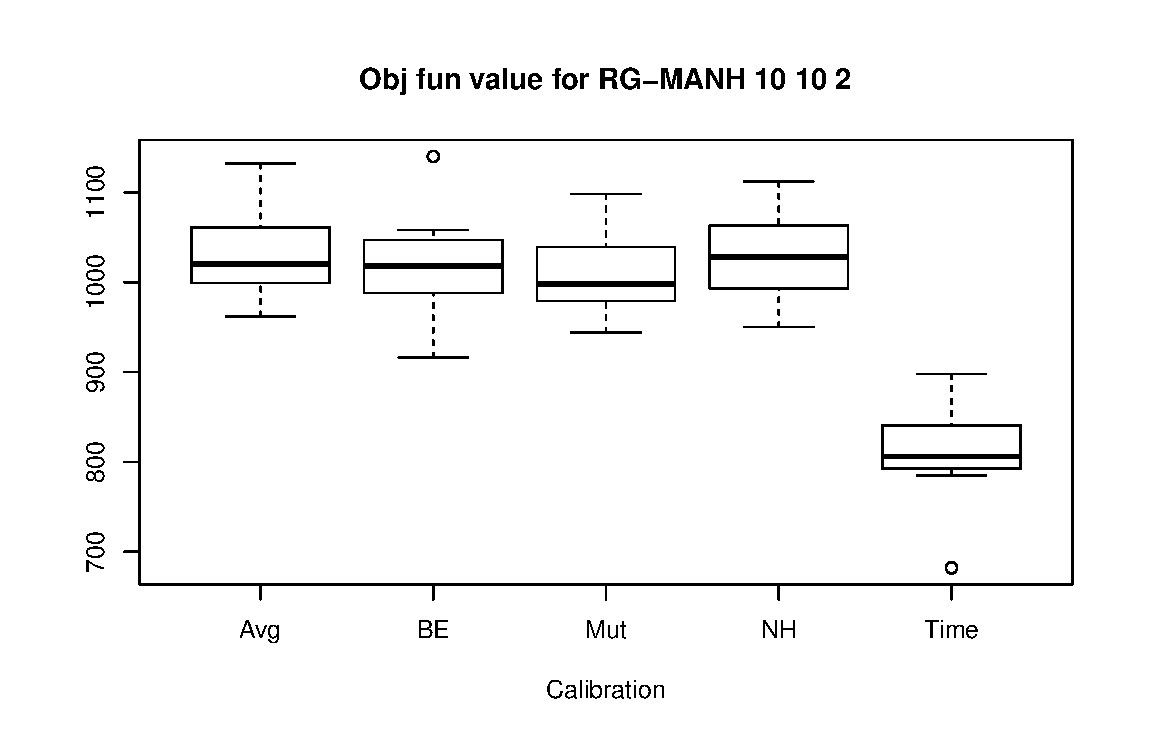
\includegraphics[scale=.4]{pics/boxplots/rg-manh-10-10-2.eps}}
\end{minipage}%
\begin{minipage}{.5\linewidth}
\centering
\subfloat[]{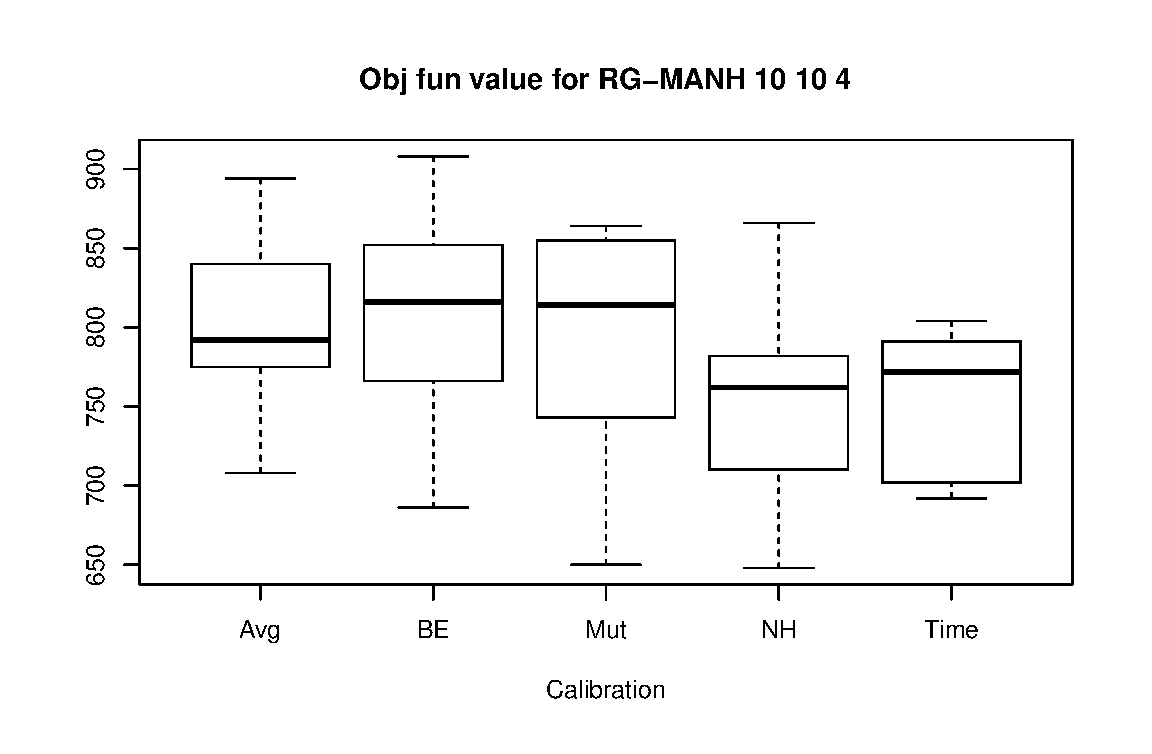
\includegraphics[scale=.4]{pics/boxplots/rg-manh-10-10-4.eps}}
\end{minipage}\par\medskip
\centering
\begin{minipage}{.5\linewidth}
\centering
\subfloat[]{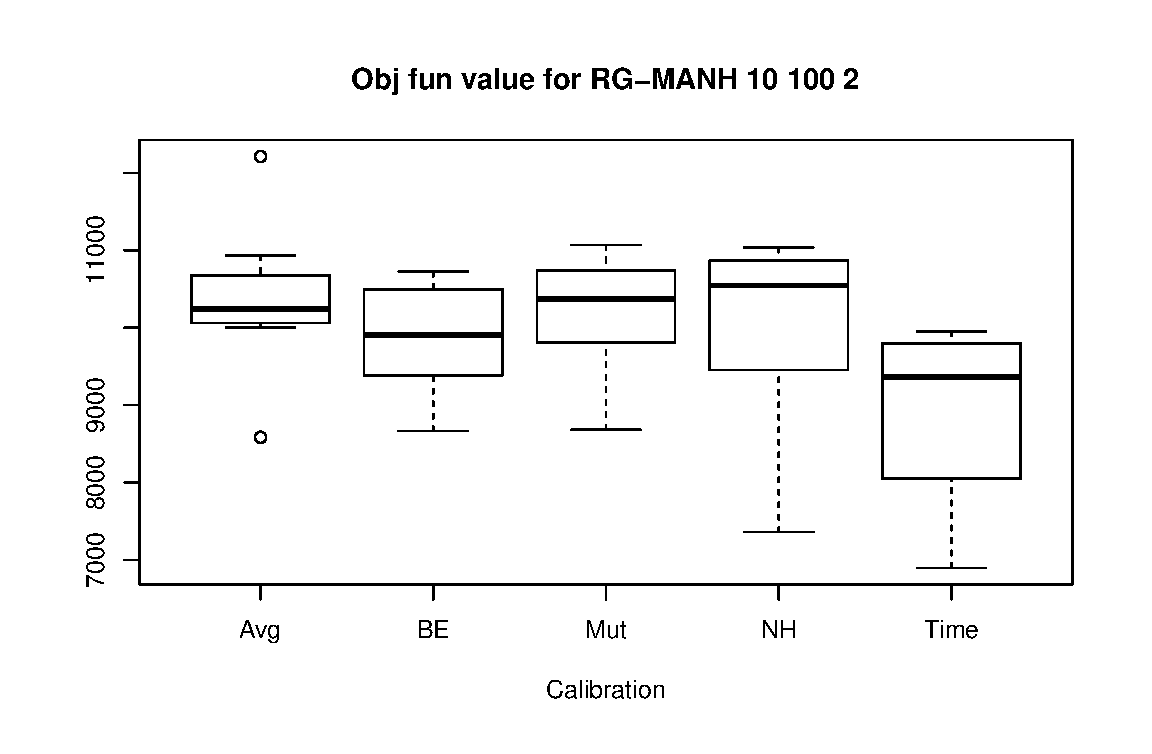
\includegraphics[scale=.4]{pics/boxplots/rg-manh-10-100-2.eps}}
\end{minipage}%
\begin{minipage}{.5\linewidth}
\centering
\subfloat[]{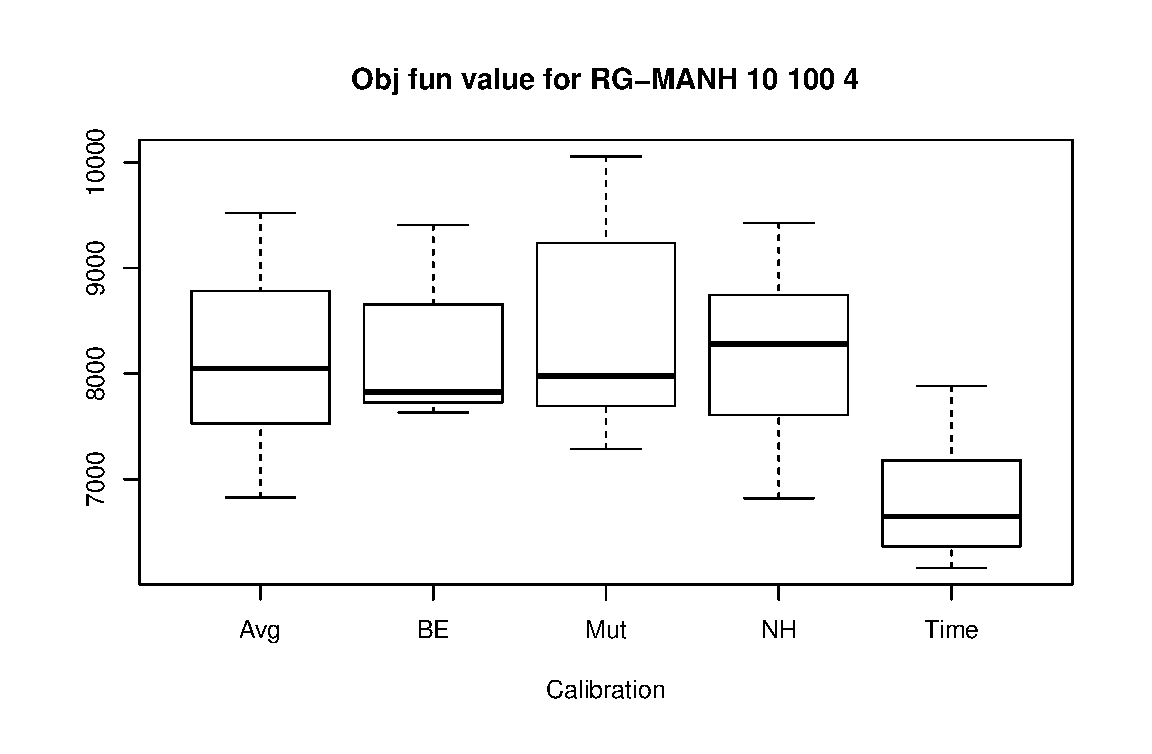
\includegraphics[scale=.4]{pics/boxplots/rg-manh-10-100-4.eps}}
\end{minipage}\par\medskip

\caption{Objective function performance for Random Grid Uniform (Manhattan
  distance) with 10 holes}
\label{fig:obj-fixed}
\end{figure}


%%%%%%%%%%%%%%%%%%%
%% RG MANH 50 holes
%%%%%%%%%%%%%%%%%%%

\begin{figure}[H]

\begin{minipage}{.5\linewidth}
\centering
\subfloat[]{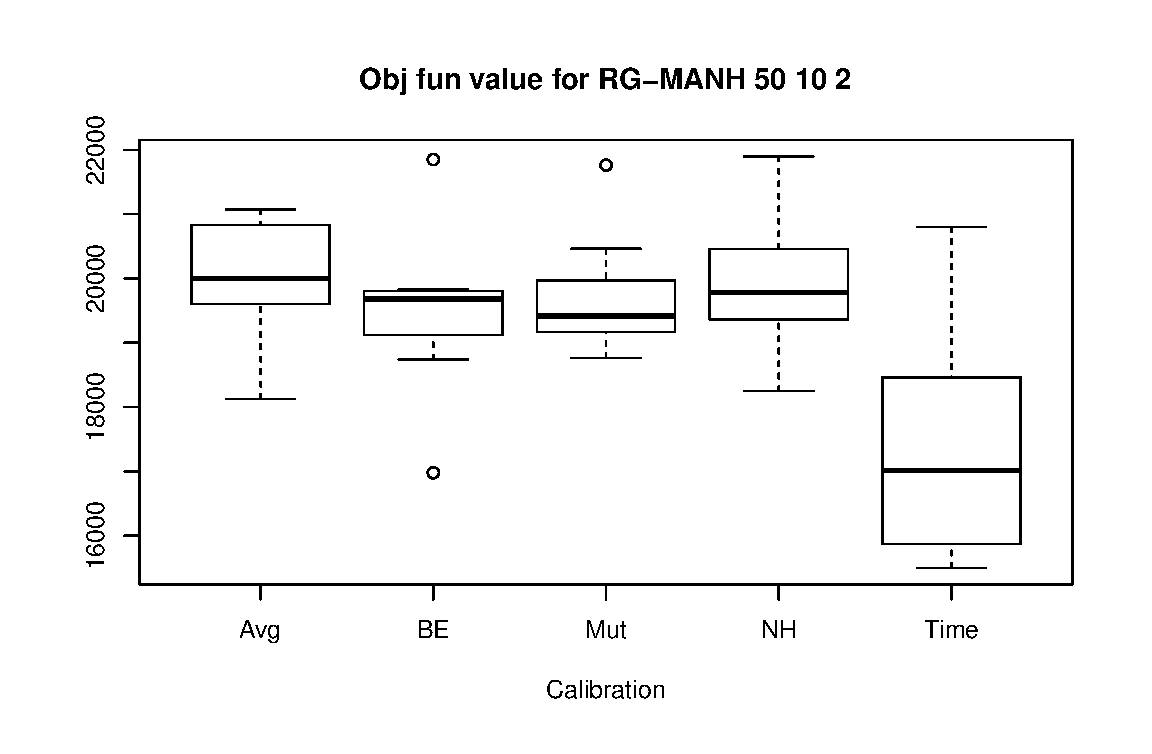
\includegraphics[scale=.4]{pics/boxplots/rg-manh-50-10-2.eps}}
\end{minipage}%
\begin{minipage}{.5\linewidth}
\centering
\subfloat[]{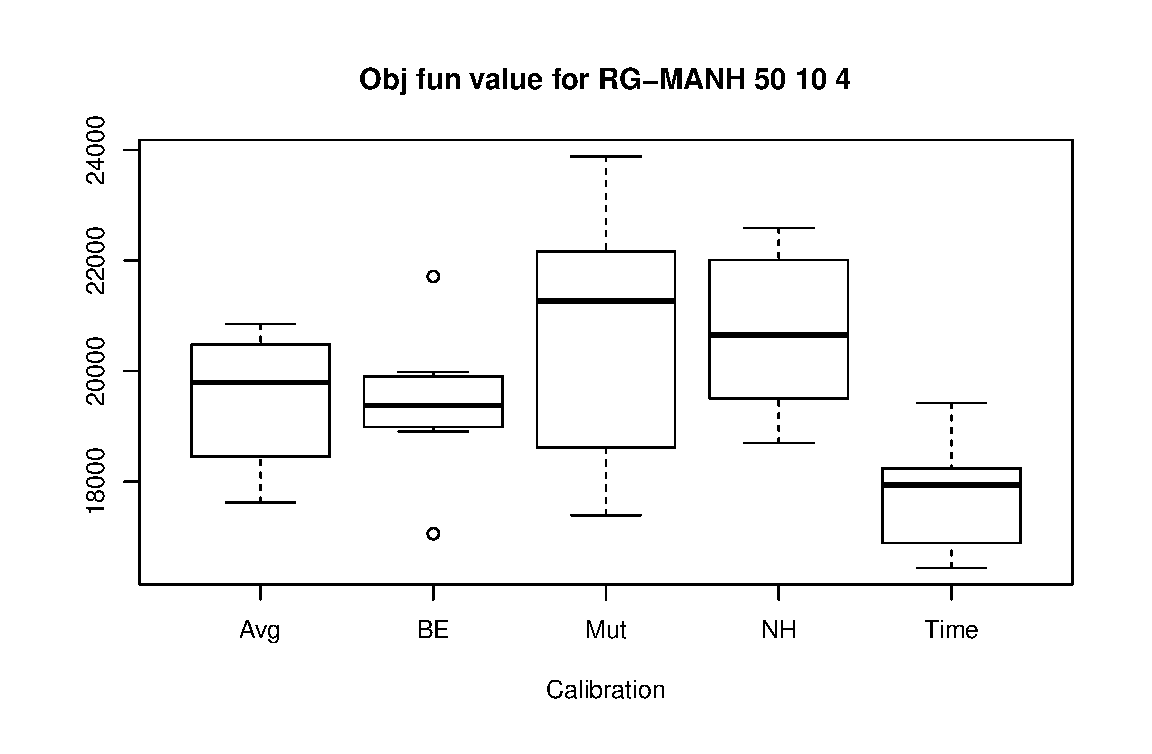
\includegraphics[scale=.4]{pics/boxplots/rg-manh-50-10-4.eps}}
\end{minipage}\par\medskip
\centering
\begin{minipage}{.5\linewidth}
\centering
\subfloat[]{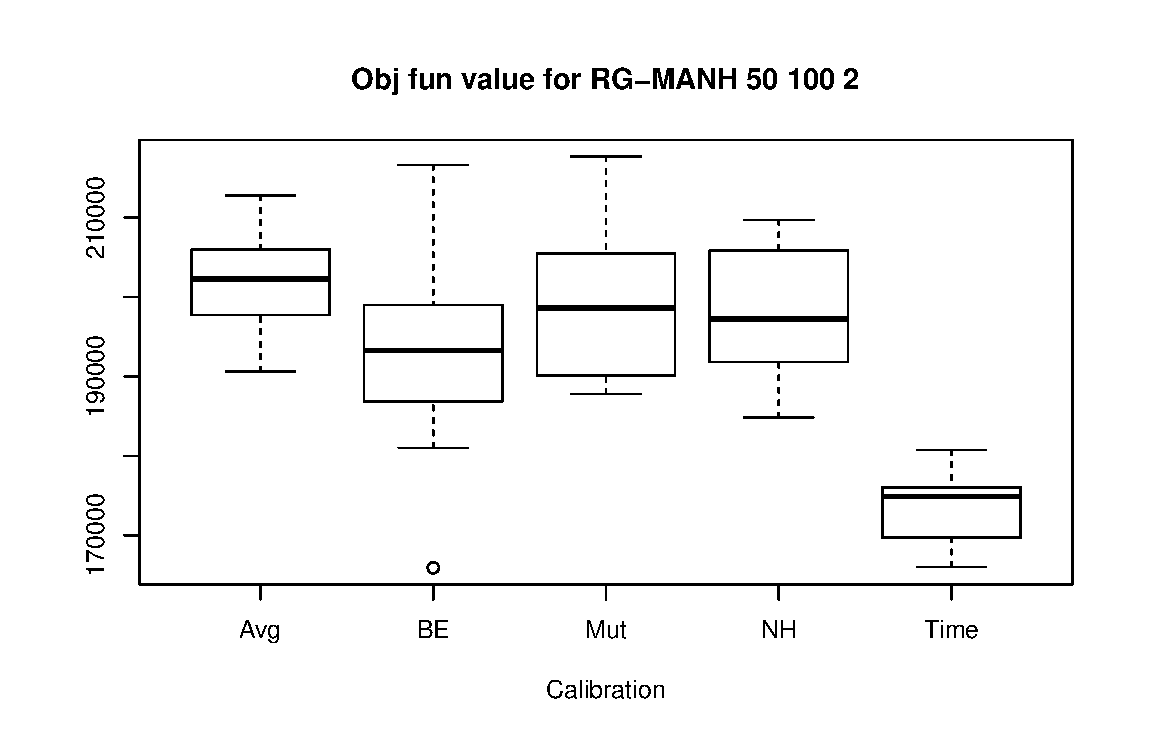
\includegraphics[scale=.4]{pics/boxplots/rg-manh-50-100-2.eps}}
\end{minipage}%
\begin{minipage}{.5\linewidth}
\centering
\subfloat[]{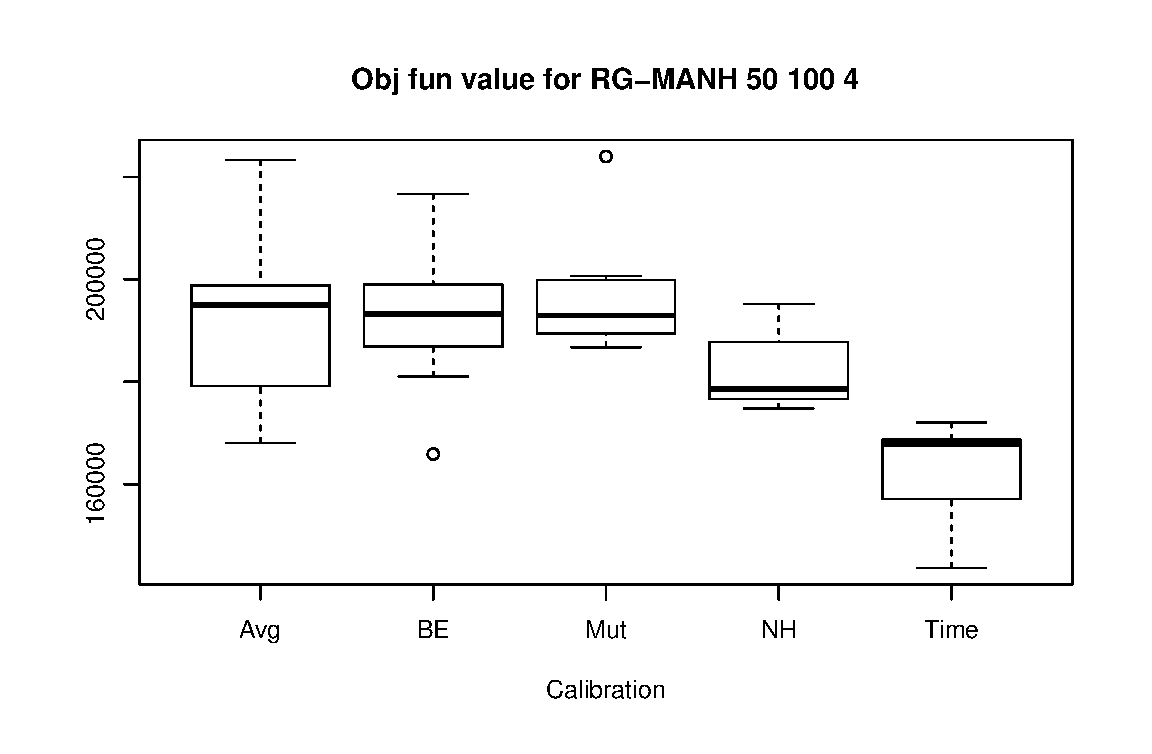
\includegraphics[scale=.4]{pics/boxplots/rg-manh-50-100-4.eps}}
\end{minipage}\par\medskip

\caption{Objective function performance for Random Grid Uniform (Manhattan
  distance) with 50 holes}
\label{fig:obj-fixed}
\end{figure}

We can make some observations on this graphs:

\begin{itemize}
  \item in almost all the graphs, \textbf{Time} tuning yielded the best
    performance in terms of objective function goodness\footnote{but it was 12
    slower in terms of efficiency}, to the point that sometimes the worst
    result achieved with this calibration outscored all the other tunings;
  \item the time component effect was minor in instances which size was pretty
    small (like 10 or 12 holes). In these cases, no method beat the
    others, but an high mutation rate often lead decent scores on randomly
    generated instances;
  \item for a high number of tests, it's true that \textbf{Mut} and
    \textbf{NH} implied a low variance among the different measurings (you can
    see it because they often have the shortest whiskers);
  \item \textbf{Avg} and \textbf{BE} produced very similar values (looking at
    the plots). Thus, I may argue that the elite size is not so significant
    for the genetic algorithm I have developed as long as there is a high
    number of offspring;
  \item it's nice to see that for the more realistic configuration (i.e. the
    Gerber one), both \textbf{Avg} and \textbf{NH} had similar results. So I
    can suppose that for realistic instances having or not an initial
    population generated with Simulated Annealing is not that relevant.
\end{itemize}

As we can see, it clearly emerges from the boxplots that the time component
has a definitely strong impact on the goodness on the solution.
